\section{An exact embedded realization}\label{sec:embedding}

We now turn the nonzero tube family of Section~\ref{sec:tubes} into a
closed exact embedded Lagrangian. A sphere factor records the direction
of the vertical gradient. Its momenta separate branches except in one
direction, and a scale varying over $S^9$ separates the remaining pairs.

We first recall the elementary generating-family criterion, including the immersion statement needed below. If $M$ is a smooth manifold, a smooth function $F:M\times\R^r\to\R$ is a \emph{Morse family} when zero is a regular value of the full map $d_wF:M\times\R^r\to(\R^r)^*$. Individual fiber Hessians need not be invertible. Write
\[
 \Crit(F)=\{(q,w):d_wF(q,w)=0\},\qquad
 \Gamma_F(q,w)=(q,d_qF(q,w)).
\]

\begin{lemma}\label{lem:generating-map}
For a Morse family, $\Gamma_F:\Crit(F)\to T^*M$ is an exact Lagrangian immersion, with primitive $F|_{\Crit(F)}$.
\end{lemma}

\begin{proof}
The critical locus is smooth of dimension $\dim M$. In local coordinates, its defining differential is the surjective matrix
\[
 A=(F_{wq},F_{ww}).
\]
A tangent vector killed by $d\Gamma_F$ has $\delta q=0$, $F_{ww}\delta w=0$, and $F_{qw}\delta w=0$. Since $F_{ww}$ is symmetric, these equations say $A^{\mathsf T}\delta w=0$. Surjectivity of $A$ forces $\delta w=0$. Thus $\Gamma_F$ is an immersion. On the critical locus $d_wF=0$, and hence
\[
 \Gamma_F^*\lambda=d(F|_{\Crit(F)}).
\]
Its pullback of $d\lambda$ is zero. The dimension just computed proves that the immersion is Lagrangian.
\end{proof}

Take the family $g_b$ from Lemma~\ref{lem:localized-family}, with $B=S^9$, $N=2m$, and a height function $\theta:B\to\R$. Fix a metric on $B$. Choose a union $U_0$ of neighborhoods of the two critical points of $\theta$ on which $g_b$ is the fixed quadratic form. Thus
\[
 \delta_0:=\min_{B\setminus U_0}\norm{d\theta}>0.
\]
Smooth angular dependence and homogeneity give a constant $C_1$ such that
\begin{equation}\label{eq:mixed-derivative-bound}
 \norm{d_wd_bg_b(w)}\leq C_1\norm{w}.
\end{equation}
Here $d_bg_b$ is a covector at $b$ and the norm is the corresponding operator norm. Its extension at $w=0$ is $C^1$, with derivative zero there.

\begin{proposition}\label{prop:embedded-realization}
On $Q=B\times S^{N-1}$ there is a smooth Morse family $F:Q\times\R^N\to\R$ which equals $g_b(w)$ outside a uniform vertical ball and whose generating map is a diffeomorphism from its critical locus onto a closed exact embedded Lagrangian $L\subset T^*Q$. Its critical locus, and hence $L$, is diffeomorphic to $Q$. The infinity class on each slice $B\times\{v_0\}$ is the chosen class $a$.
\end{proposition}

\begin{proof}
Choose
\begin{equation}\label{eq:scale-choice}
 K\delta_0>C_1/c,
\end{equation}
where $c\norm{w}\leq\norm{\nabla g_b(w)}\leq C\norm{w}$. Set
\[
 R(b)=\Lambda e^{K\theta(b)}.
\]
Let $G_b$ be smooth on all of $\R^N$ and agree with $g_b$ for $\norm{w}\geq1$; multiplying by a radial cutoff which vanishes near zero gives such a family. Let $\beta:[0,\infty)\to[0,1]$ be smooth, equal to one on $[0,1]$ and zero on $[2,\infty)$. Define
\begin{equation}\label{eq:embedded-family}
 F(b,v,w)=G_b(w)-R(b)\beta(\norm{w}/T)\langle v,w\rangle,
 \qquad v\in S^{N-1}.
\end{equation}
Choose $\Lambda$ so large that
\[
 R_{\min}>\max\left\{C,\ \sup_{b,\,\norm{w}\leq1}\norm{\nabla G_b(w)}\right\}.
\]
With
\[
 D_\beta=\sup_{s\geq0}\bigl(\abs{\beta(s)}+s\abs{\beta'(s)}\bigr),
\]
choose
\begin{equation}\label{eq:T-choice}
 T>\max\{1,R_{\max}/c,D_\beta R_{\max}/c\}.
\end{equation}
These choices are made in the order $K$, $\Lambda$, $T$.

There are no vertical critical points with $\norm{w}\leq1$, by the choice of $R_{\min}$. For $\norm{w}\geq T$, the vertical derivative of the cutoff linear term has norm at most $D_\beta R(b)$, so
\[
 \norm{d_wF}\geq c\norm{w}-D_\beta R(b)>0.
\]
All critical points therefore satisfy precisely
\begin{equation}\label{eq:embedded-critical}
 \nabla g_b(w)=R(b)v.
\end{equation}
Conversely every solution of this equation has
\[
 1<R(b)/C\leq\norm{w}\leq R(b)/c<T,
\]
so it is a critical point of~\eqref{eq:embedded-family}. By homogeneity, the critical locus is smoothly parameterized by
\begin{equation}\label{eq:critical-parametrization}
 (b,u)\longmapsto
 \left(b,\frac{\nabla g_b(u)}{\norm{\nabla g_b(u)}},
 \frac{R(b)u}{\norm{\nabla g_b(u)}}\right),
 \qquad u\in S^{N-1}.
\end{equation}
Its inverse recovers $u=w/\norm{w}$.

To check regularity of the critical equation, vary $v$ in $v^\perp$: its contribution to the differential is $-R\delta v$. Radial variation $\delta w=w$ contributes $\nabla g_b(w)=Rv$, because $\nabla g_b$ is homogeneous of degree one. These variations span $\R^N$. Hence $F$ is a Morse family, and Lemma~\ref{lem:generating-map} gives an exact Lagrangian immersion.

It remains to prove injectivity. Two points with the same image must first have the same base coordinates $(b,v)$. At critical points the cutoffs are constant and $G_b=g_b$. Equality of the covectors in the sphere direction, which are
\[
 d_vF(\dot v)=-R(b)\langle w,\dot v\rangle,
 \qquad \dot v\perp v,
\]
therefore implies $w-w'=tv$ for some $t\in\R$. Both endpoints, and their whole straight segment, have norm at most $R(b)/c$. The bound~\eqref{eq:mixed-derivative-bound} yields
\begin{equation}\label{eq:collision-bound}
 \norm{d_bg_b(w)-d_bg_b(w')}
 \leq (C_1/c)R(b)\abs{t}.
\end{equation}
This use of the fundamental theorem of calculus remains valid if the segment passes through zero, since $d_bg_b$ is $C^1$ there.

The difference in the $B$-momenta is
\[
 d_bg_b(w)-d_bg_b(w')-KR(b)t\,d\theta_b.
\]
For $b\notin U_0$, its norm is at least
\[
 R(b)\abs{t}\bigl(K\delta_0-C_1/c\bigr).
\]
By~\eqref{eq:scale-choice}, equality of those momenta forces $t=0$. For $b\in U_0$, the function $g_b$ is the fixed nondegenerate quadratic form, and~\eqref{eq:embedded-critical} already has a unique solution for each $v$. Thus the immersion is injective everywhere.

Figure~\ref{fig:momentum-separation} summarizes the two momentum tests.
\begin{figure}[tbp]
\centering
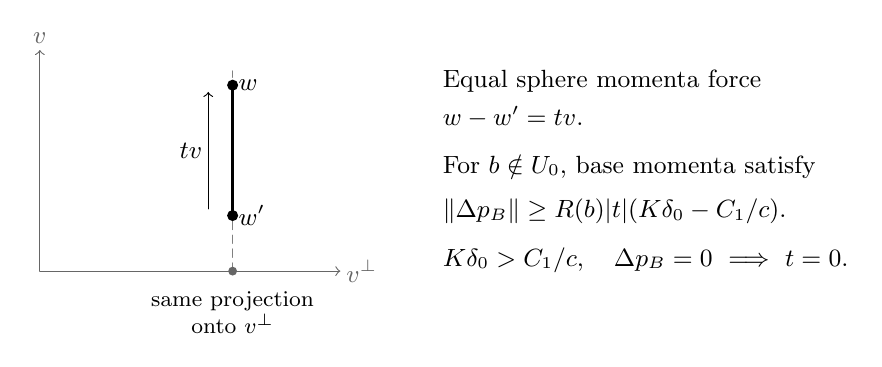
\begin{tikzpicture}[x=0.72cm,y=0.72cm,font=\small,
  every node/.style={inner sep=2pt},line cap=round]
  \draw[->,black!60] (0,0.5)--(5.3,0.5) node[right] {$v^\perp$};
  \draw[->,black!60] (0,0.5)--(0,4.4) node[above] {$v$};
  \draw[densely dashed,black!50] (3.4,0.5)--(3.4,4.03);
  \draw[line width=1pt] (3.4,1.48)--(3.4,3.78);
  \fill (3.4,1.48) circle (2pt) node[right] {$w'$};
  \fill (3.4,3.78) circle (2pt) node[right] {$w$};
  \draw[->] (2.97,1.6)--(2.97,3.66)
    node[midway,left] {$tv$};
  \fill[black!60] (3.4,0.5) circle (1.6pt);
  \node[anchor=north,align=center,font=\footnotesize] at (3.4,0.24)
    {same projection\\onto $v^\perp$};
  \node[anchor=west] at (7,3.85) {Equal sphere momenta force};
  \node[anchor=west] at (7,3.22) {$w-w'=tv$.};
  \node[anchor=west] at (7,2.35) {For $b\notin U_0$, base momenta satisfy};
  \node[anchor=west] at (7,1.55)
    {$\|\Delta p_B\|\geq R(b)|t|(K\delta_0-C_1/c)$.};
  \node[anchor=west] at (7,0.7)
    {$K\delta_0>C_1/c,\quad \Delta p_B=0\ \Longrightarrow\ t=0$.};
\end{tikzpicture}
\caption{Schematic of the two momentum tests for two critical points at
fixed base coordinates $(b,v)$, with $\Delta p_B$ the difference of the $B$-momenta. Sphere
momenta detect the component of $w$ perpendicular to $v$; the varying
scale separates the remaining pairs outside $U_0$.
Within $U_0$, the fixed quadratic critical equation has a unique solution.
The two-dimensional drawing represents an orthogonal decomposition only.
The estimate also holds when the segment from $w'$ to $w$ passes through
zero.}
\label{fig:momentum-separation}
\end{figure}


The parameter space in~\eqref{eq:critical-parametrization} is compact and has no boundary. A compact injective immersion is an embedding, so its image is a closed exact embedded $L\cong Q$. In fact Euler's identity gives the global primitive $F|_{\Crit(F)}=-g_b(w)$, although the exactness argument did not require this formula. Finally, for $\norm{w}\geq2T$, the family equals $g_b(w)$ independently of $v$. Its restriction at infinity to any fixed sphere slice therefore represents $a$.
\end{proof}
